% Created 2019-06-06 Thu 14:25
% Intended LaTeX compiler: pdflatex
\documentclass{article}
\usepackage[utf8]{inputenc}
\usepackage[T1]{fontenc}
\usepackage{graphicx}
\usepackage{grffile}
\usepackage{longtable}
\usepackage{wrapfig}
\usepackage{rotating}
\usepackage[normalem]{ulem}
\usepackage{amsmath}
\usepackage{textcomp}
\usepackage{amssymb}
\usepackage{capt-of}
\usepackage{hyperref}
\author{Carolina Silva, Cristina Pinto, João Fraga}
\date{\today}
\title{Projeto de Sistemas Operativos}
\hypersetup{
 pdfauthor={Carolina Silva, Cristina Pinto, João Fraga},
 pdftitle={Projeto de Sistemas Operativos},
 pdfkeywords={},
 pdfsubject={},
 pdfcreator={Emacs 26.2 (Org mode 9.2.3)},
 pdflang={English}}
\begin{document}

\maketitle
\maketitle

\pagebreak{}
\tableofcontents
\listoffigures
\listoftables

\pagebreak{}
\section{Introdução}
\label{sec:org5d4b4bd}

Este trabalho \cite{enunciado} tem como objetivo o desenvolvimento de uma estrutura de dados sincronizada para ser utilizada numa aplicação servidor e cliente.
O projeto \cite{enunciado} tem também como objetivos o desenvolvimento de um servidor de ficheiros, que deverá usar multithreading para atender clientes em simultâneo, e uma aplicação para clientes, onde podem inserir, visualizar e apagar mensagens contidas em filas.

Assim, no servidor, foram desenvolvidos os ficheiros server.h (onde estão contidos todos os protótipos das funções associadas ao servidor) e server.c (onde está o programa principal do servidor e as funções referentes ás threads, lists e ao funcionamento do próprio servidor e o menu principal).

No Cliente,  foram desenvolvidos os ficheiros client.h (com os protótipos de funções) e client.c (onde se encontra o programa principal, bem como as funções connect, getmenu, dowhile, sendoption e parseoutput.

Como suporte para o desenvolvimento deste trabalho, recorremos aos materiais fornecidos pelo docente da unidade curricular, bem como a bibliografia de referência sugerida para esta disciplina.

\pagebreak{}
\section{Estrutura do projeto}
\label{sec:org602821f}

\begin{figure}[htbp]
\centering
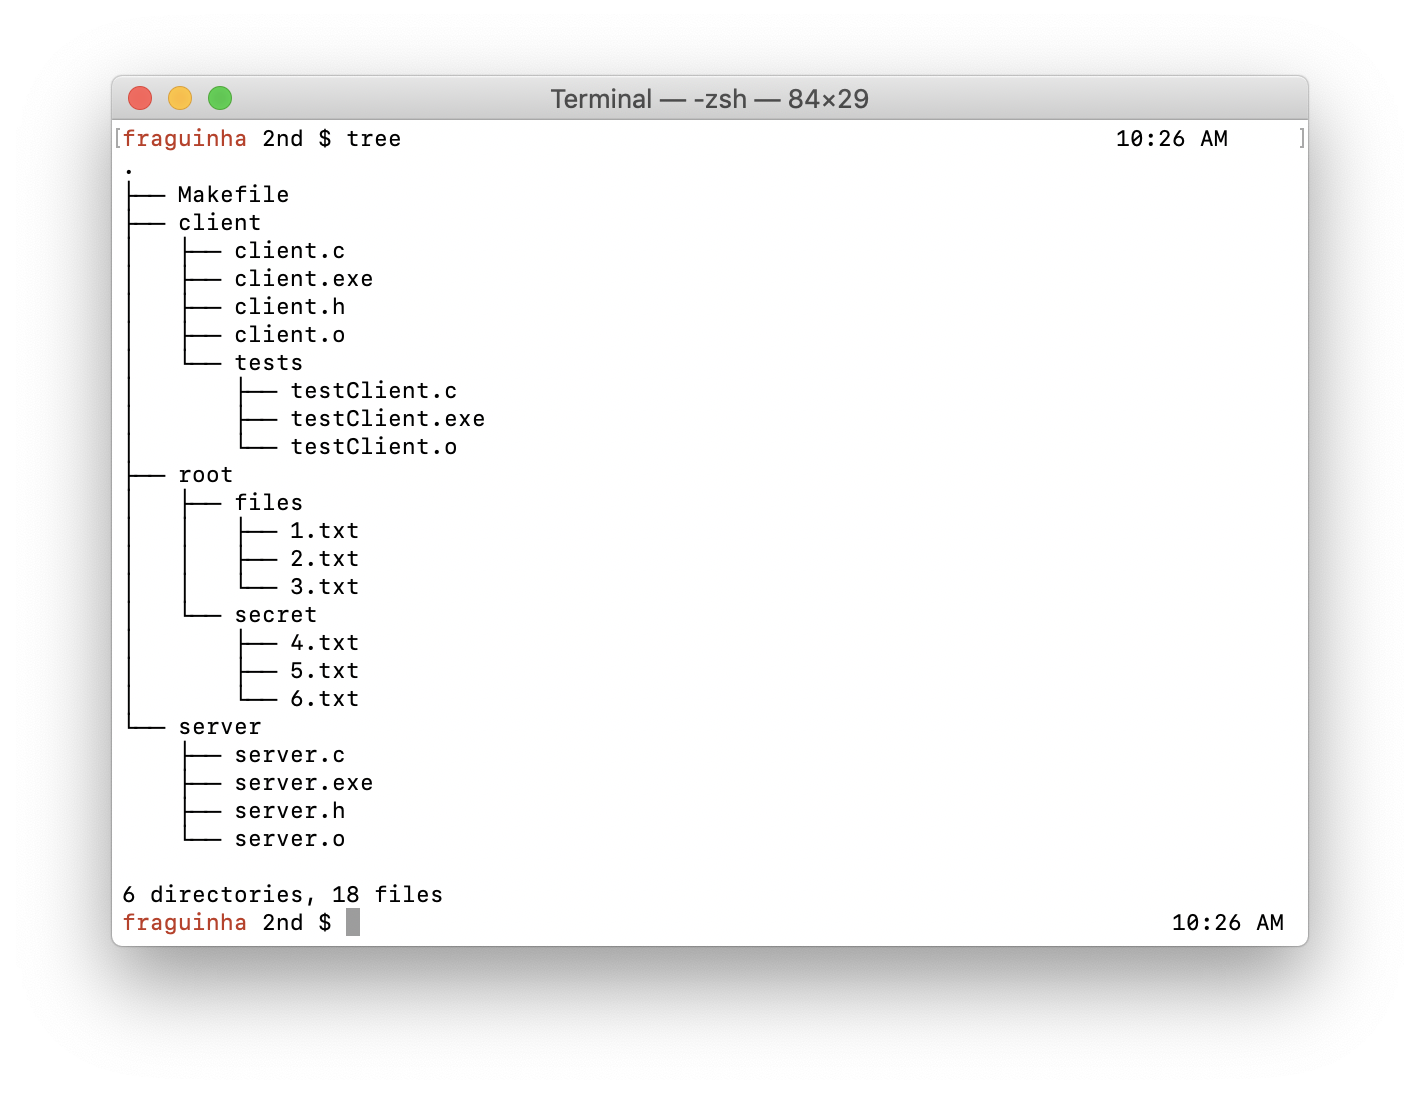
\includegraphics[width=.9\linewidth]{./img/estrutura.png}
\caption{\label{fig:estrutura}
Estrutura de ficheiros do projeto}
\end{figure}

O projeto está dividido em 3 pastas principais: root, client e server.

A pasta root é a pasta raiz da funcionalidade de tratamento de ficheiros do nosso servidor.
Esta pasta contém duas subpastas (files e secret) que por sua vez contêm ficheiros sem, ou, com password respetivamente.

A pasta client contém todo o código relativo ao programa cliente e uma subpasta tests com código relativo aos testes automaticos.

A pasta server contém todo o código relativo ao programa servidor.

\pagebreak{}
\section{Cliente}
\label{sec:org4c5ab82}

\subsection{Abordagem de cliente}
\label{sec:orgf8a1779}

Durante a realização do nosso projeto decidimos fazer do cliente um programa "dumb" que apenas interpreta mensagens do servidor e pede input ao utilizador, não efectuando nenhum processamento local.

\subsection{Client}
\label{sec:org47b48db}

Este programa vai permitir a um cliente interagir com o servidor.

\begin{figure}[htbp]
\centering
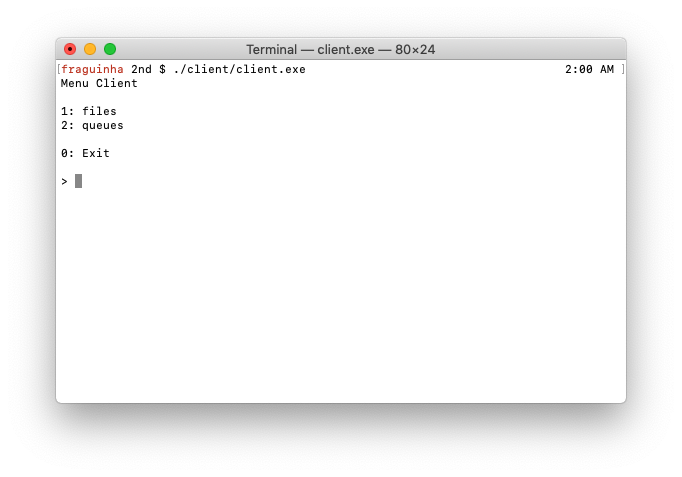
\includegraphics[width=.9\linewidth]{./img/mainmenu.png}
\caption{\label{fig:estrutura}
Menu principal}
\end{figure}

\begin{figure}[htbp]
\centering
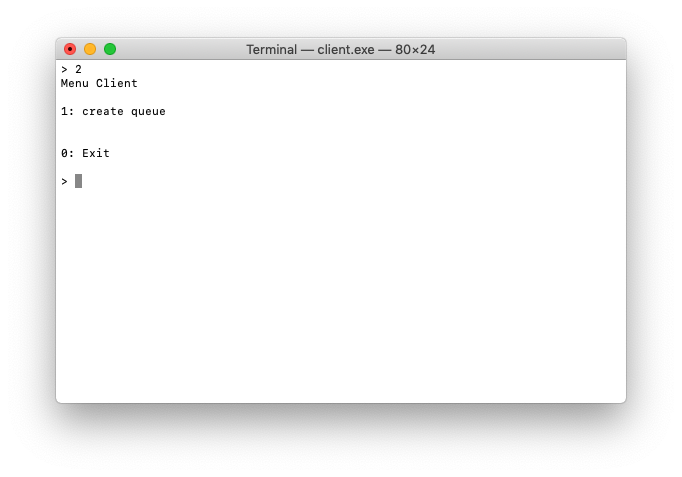
\includegraphics[width=.9\linewidth]{./img/queue1.png}
\caption{\label{fig:queue1}
Menu queue sem listas criadas}
\end{figure}

\begin{figure}[htbp]
\centering
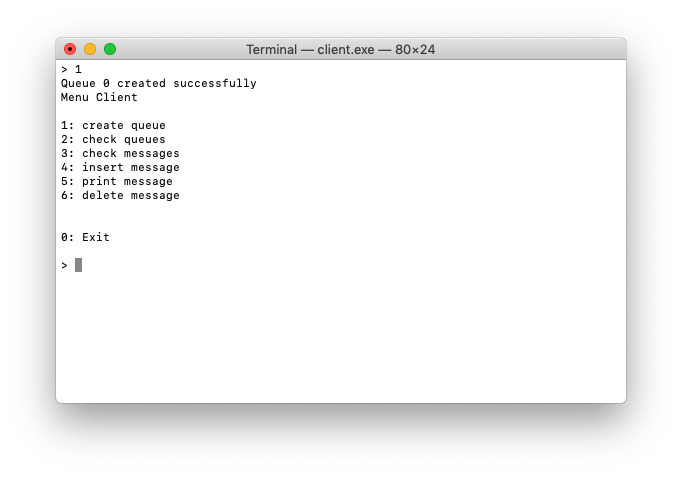
\includegraphics[width=.9\linewidth]{./img/queue2.png}
\caption{\label{fig:queue2}
Menu queue com listas criadas}
\end{figure}

\subsubsection{connect}
\label{sec:org5859cbe}

Vai permitir ao cliente aceder a informação do pipe individual que o servidor estabelece para ele.

\subsubsection{get menu}
\label{sec:org154afbc}

Esta função vai permitir que o cliente tenha acesso ao menu inicial.

\subsubsection{do while}
\label{sec:org053cdf9}

Esta função vai imprimir continuamente menus e faz chamadas ao send options.

\subsubsection{send options}
\label{sec:orgabf89f1}

Vai estar a tratar continuamente o que vai ser necessário enviar ao cliente, fazendo uso de uma função auxiliar parse output.

\subsubsection{parse output}
\label{sec:org747d66f}

Esta função vai fazer a interpretação de comandos enviados pelo servidor.

\begin{table}[htbp]
\caption{\label{tab:messages}
Mensagens a receber do servidor e as suas respectivas descrições}
\centering
\begin{tabular}{ll}
\hline
Mensagens & Descrição\\
\hline
id & Esta mensagem é utilizada para pedir ao utilizador o id de uma fila\\
idp & Esta mensagem é utilizada para pedir o id de uma mensagem\\
filename & Esta mensagem é utilizada para pedir o nome de um ficheiro\\
message & Esta mensagem é utilizada para pedir uma mensagem para uma lista\\
password & Esta mensagem é utilizada para pedir a password dos ficheiros secretos\\
invalid & Esta mensagem é utilizada para indicar uma opção invalida\\
print & Esta mensagem é utilizada para indicar o envio de informação a imprimir\\
error & Esta mensagem é utilizada para indicar a occorência de um erro\\
file & Esta mensagem é utilizada para indicar o envio do conteúdo de um ficheiro a imprimir\\
\hline
\end{tabular}
\end{table}

\subsubsection{read file \cite{Chapter10}}
\label{sec:org1ad2619}

Esta função vai ler o ficheiro pedido até ao fim.

\pagebreak{}
\section{Servidor}
\label{sec:orgb856bcf}

\subsection{Threads \cite{Chapter9}}
\label{sec:orgf777310}

\begin{figure}[htbp]
\centering
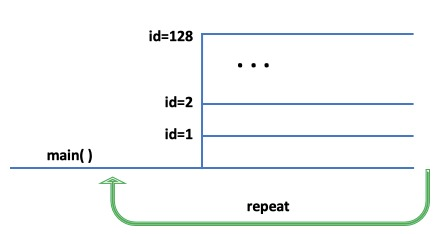
\includegraphics[width=.9\linewidth]{./img/threads.jpeg}
\caption{\label{fig:threads}
Esquema de threads}
\end{figure}

Neste trabalho efetuou-se uma abordagem de um servidor multithreaded, em que para cada pedido de conecção de um cliente é criada uma thread para servir o mesmo.

De modo a garantir o constante funcionamento do servidor foi necessário ignorar os broken pipes obtidos quando um cliente termina.
Para isto utilizou-se a função signal(SIGPIPE,  SIG IGN). \cite{signal2}
Assim foi possível realizar o unlink dos pipes estabelecidos com essa thread não causando problemas no servidor.

\subsection{Primeira comunicação}
\label{sec:orgf07063a}

\begin{figure}[htbp]
\centering
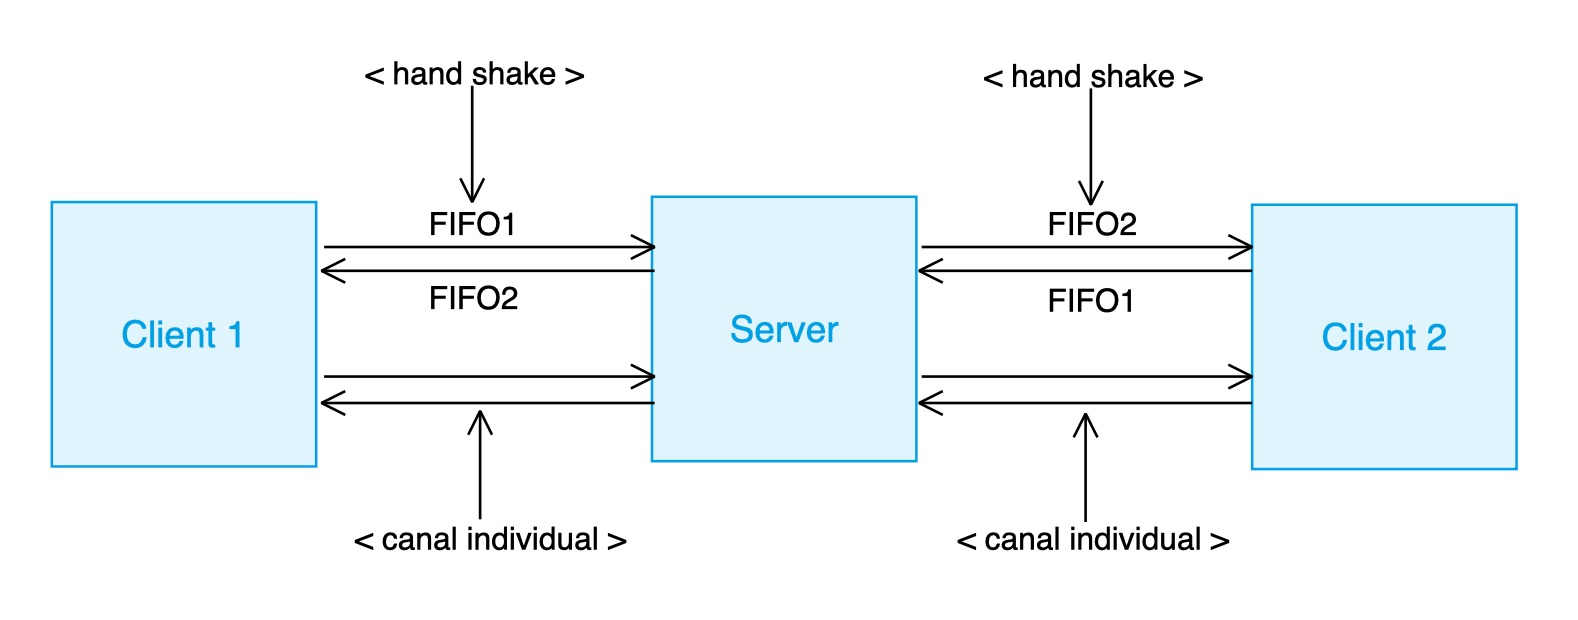
\includegraphics[width=.9\linewidth]{./img/handshake.jpeg}
\caption{\label{fig:handshake}
Comunicação inicial entre clientes e servidores \cite{Chapter11} \cite{Chapter12}}
\end{figure}

Inicialmente os clientes utilizam um pipe comum (FIFO1 \& FIFO2) para se conectarem ao servidor e realizarem um handshake.
O servidor utiliza este pipe para informar os clientes sobre quais os novos fifos a utilizar.
Deste modo as comunicações realizadas entre um cliente e o servidor são efectuadas através de um pipe privado.

\subsection{Main}
\label{sec:org8837ab5}

Esta é a função principal do servidor a partir da qual o mesmo começa a execução.
Aqui corre um loop infinito onde são descobertas conecções e criadas threads para lidar com as mesmas. \cite{Chapter9}

\subsection{Server}
\label{sec:orgb7f6e05}

Esta função vai executar a thread individual de cada cliente, e permite que o cliente possa usufruir de todas as funcionalidades do servidor.
O servidor terá a função de informar o cliente sobre as opções que este pode tomar e age de acordo.

\subsection{Protocolo de comunicação}
\label{sec:org911493c}

\begin{figure}[htbp]
\centering
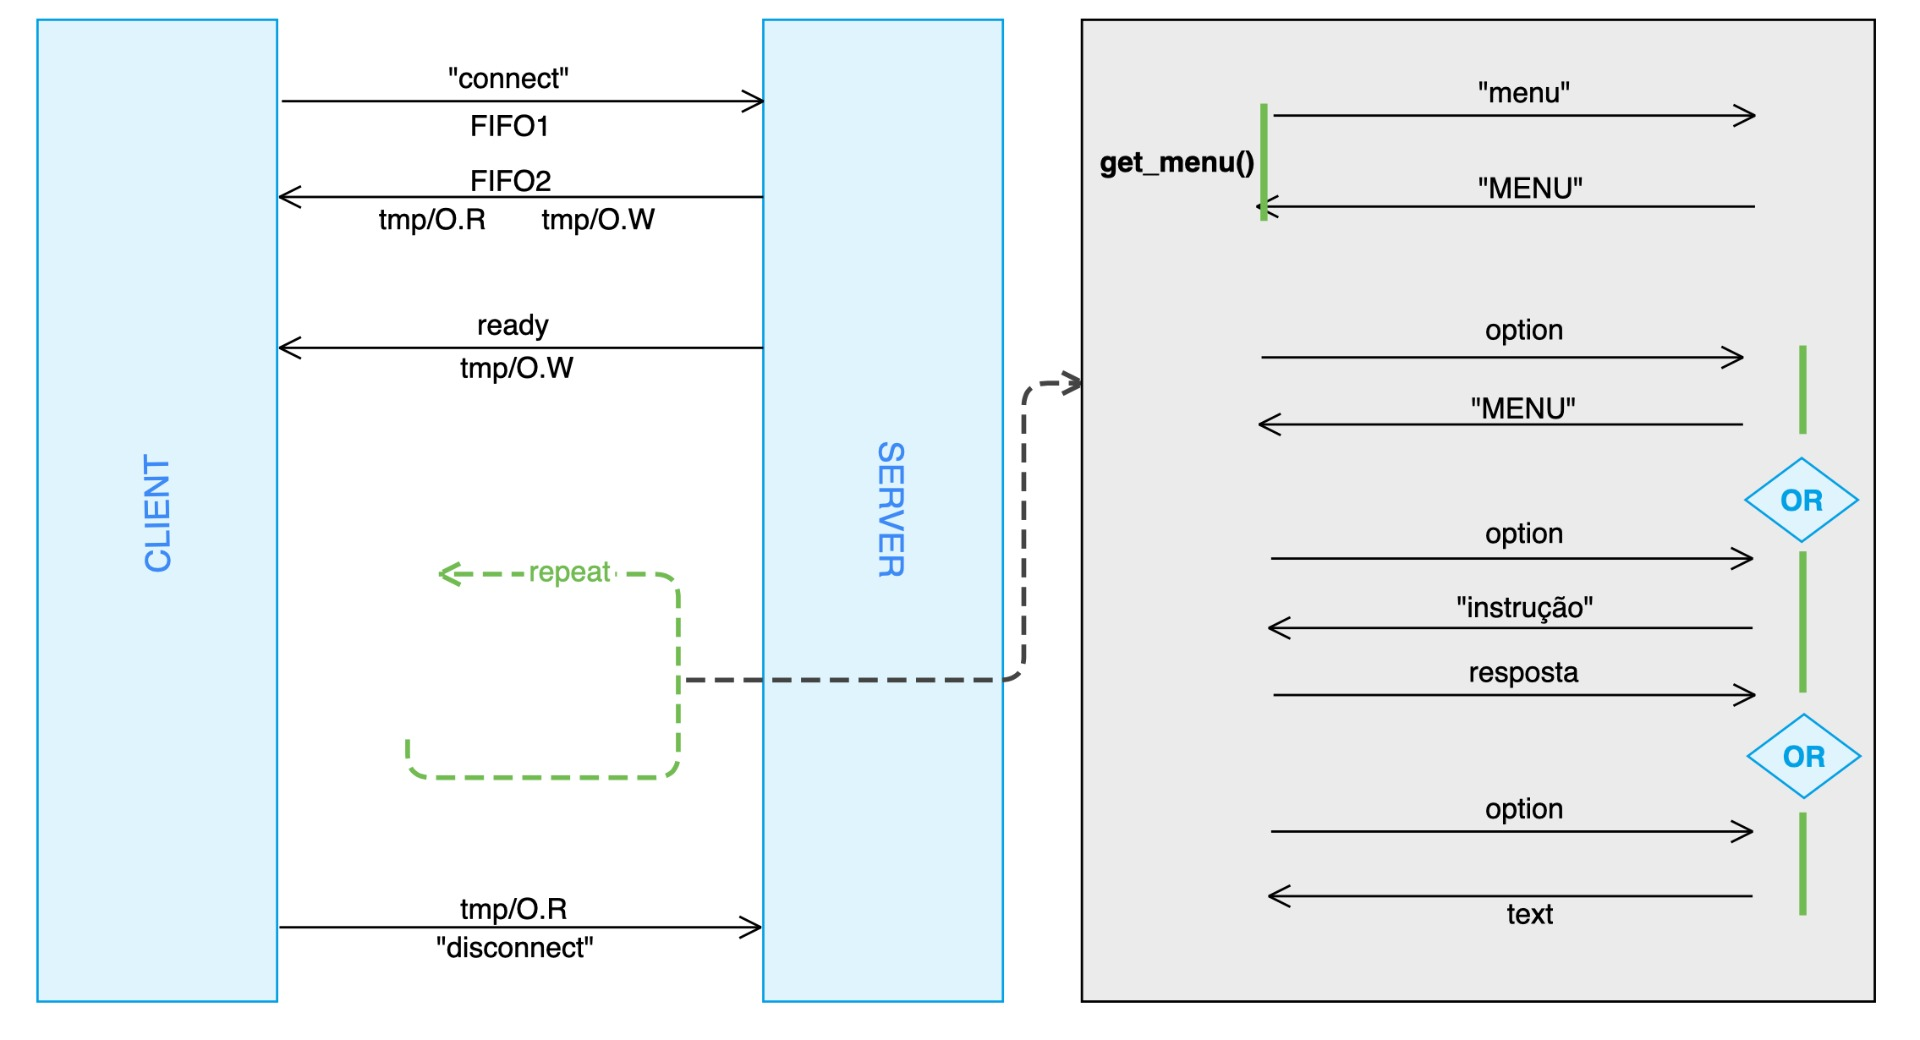
\includegraphics[width=.9\linewidth]{./img/protocol.jpeg}
\caption{\label{fig:protocol}
Protocolo de comunicação um cliente e o servidor}
\end{figure}

Após o handshake inicial e a criação de um canal de comunicação privado, a comunicação entre o cliente e o servidor inicia-se com um pedido do menu por parte do cliente.
O servidor responde com o menu inicial.

Conforme as opções tomadas pelo utilizador o servidor poderá fornecer novos menus, enviar mensagens de resposta e solicitar o envio de informação.

\subsection{Listas}
\label{sec:orga06e493}

\subsubsection{funções auxiliares}
\label{sec:org57526e5}

Implementamos algumas funções auxiliares que serão utilizadas na execução de outras funções principais, nomedamante:
\begin{itemize}
\item make node
\item push
\item pop
\item is empty list
\item print list
\item count list
\item print message list
\end{itemize}

\subsubsection{server queue}
\label{sec:org294ee08}

Esta é a função a partir da qual são selecionadas todas as funcionalidades referentes ás filas.
O servidor apenas apresenta as opções que se encontram disponiveis para ultilização pelo cliente.

Todas estas funções fazem uso de um lock para se manterem sincronizadas. \cite{Chapter13}

\begin{enumerate}
\item create queue
\label{sec:org6b36f13}

Esta função vai permitir criar uma fila.

\item check queue
\label{sec:orgf7fe930}

Esta função vai mostrar quais são os IDs das fila que existem.

\item check messages
\label{sec:org93ceaaf}

Esta função vai permitir mostrar os IDs das mensagens de uma determinada fila.

\item insert message
\label{sec:org14bbe7c}

Esta função vai verificar se o ID é válido e insere a mensagem na fila correspondente.

\item print message
\label{sec:orgf09f3bc}

Esta função imprime uma mensagem com um determinado ID de uma determinadas lista.

\item delete message
\label{sec:org58882b8}

Esta função vai apagar uma mensagem de uma determinada lista.
\end{enumerate}

\subsection{Ficheiros}
\label{sec:org33eb065}

\subsubsection{server file}
\label{sec:orgad34d3d}

Esta é a função a partir da qual são executadas todas as funcionalidades referentes aos ficheiros. \cite{Chapter10}

É solicitado ao cliente um nome de um ficheiro e caso este exista, e lhe enviada a informação contida no ficheiro.
Se o ficheiro estiver na pasta secret, é requerido ao cliente a password.

\begin{enumerate}
\item print file
\label{sec:orgffe26d3}

Esta função vai enviar para o cliente toda a informação referente a um determinado ficheiro.

\pagebreak{}
\end{enumerate}
\section{Testes}
\label{sec:org3820134}

Este programa vai permitir fazer testes para verificar a correta implementação do servidor de filas.
Para isto, serão criadas várias threads para simular o acesso ao servidor por varios clientes. \cite{Chapter9}
Cada um destes clientes realizará várias das diferentes operações de filas em simultâneo de modo a validar a correcta implementação do servidor de filas multithreaded. \cite{Chapter9}

\pagebreak{}
\section{Conclusão}
\label{sec:org24c1a02}

O desenvolvimento deste projeto ajudou no aprofundamento de competências de Sistemas Operativos, nomeadamente no desenvolvimento, implementação e especificação de estruturas de dados clássica, utilização de listas e filas e implementações thread e multithread, bem como no desenvolvimento de um servidor aplicacional.

Assim, o desenvolvimento do projeto proposto na unidade curricular de Sistemas Operativos foi bastante enriquecedor, pois permitiu mobilizar os conteúdos apreendidos no decorrer das aulas teóricas e práticas.

\pagebreak{}
\bibliographystyle{plain}
\bibliography{refs}
\end{document}